\documentclass[../main.tex]{subfiles}
\graphicspath{{\subfix{../images/}}}
\begin{document}

In the very beginning, this pamphlet is bidding you welcome, in order to use this and the following lessons right away to learn.
This pamphlet is a guide in how to attack the task of learning.

\section{Transcription}
If you want to record verbal information in written form you have to be able to \emph{take notes in a useful manner}. Due to that reason, transcribing\index{transcription} is part of the fundamental skills of verbal communication. At the same time, it's the base for the mastery of other writing tasks, like the composing of a protocol or a process or result.
Even though modern media replaces traditional tools in a lot of ways, a notebook can't entirely replace the work with pen and paper.
If you wish to transcribe at an event (lesson, seminar, lecture,\ldots ) you don't want to have a protocol of what has been said.
Very few people would be capable of achieving this, even if they know stenography (shorthand).
There are no fixed rules for transcribing, but there are certain tested techniques form which one shouldn't deviate without good reasons.

\title{Transcribing Means Listening}

If you don't want to listen, you can't transcribe! That's the simple truth of it. This act of listening isn't passive hearing, but {true listening}. Only if your thoughts follow the material which your ears hear, you can transcribe in a useful manner.


\title{Transcribing Means Choosing}

It doesn't make any sense trying to write down as much as possible or even word by word.
If you're writing like this, you can't listen anymore and the transcription isn't meant to document verbal information.\index{learning!discerning}
The true art of transcribing is to discern meaningful form not meaningful, and between important, less important or unimportant material.
And that fact is easier to state than to apply.

\title{Transcribing Means Keeping the Overview}
In order to make a meaningful choice of information suited to transcribe it makes sense to write once the speaker completes their thought or changes to a less important topic.\index{learning!overview}
It's more productive to follow a thought to the end than to try to continuously collect the pieces of it on the go.

\title{11 Tips for Transcriptions}
Translated from~\cite{Teachsam}

\begin{enumerate}
\item Use a {lot of paper}, write only on one side. Use different sheets for overview mind maps and other notes.
\item {Listen closely} and {think along actively}.
\item To differentiate between important and unimportant material, keep the topic of the talk in mind and watch out for the {speaker's signals} (ex. remarks, summing up a section as transition, emphasis). 
\item Only start writing once a ``unit of meaning'', a thought has been conveyed. 
\item Check continuously to see that you {understand the connections} and note and expand them separately in {mind maps or structure diagrams}.
\item Write in an {economical} way: make  note only of the {essential} information.
\item Use {useful abbreviations}, which are still understandable later.
\item {Don't abbreviate names} or unknown technical terms.
\item If certain {quotations or literature references} are important, make note of  them {thoroughly}.  
\item Make note of keywords in a way that shows {connections and relations} between the different pieces of information. Use {arrows, boxes or emphasis} with a highlighter. 
\item Whenever possible, complete at least one {prior reading of the topic}, and have {questions} in mind. This makes the class lecture a review rather than a first encounter.
\end{enumerate}

\newpage
Tips for abbreviations:

\begin{itemize}
\item Write out monosyllabic words (norm, sport, bar)
\item Leave out superfluous letters (abbreviation =abrv., result = res., United States = USA.
\item Only hint to articles: the = t. 
\item Official abbreviations are kept unchanged (EU, USA, UFO)
\end{itemize}

\epigraph{Anyone who stops learning is old, whether at twenty or eighty. Anyone who keeps learning stays young.}{\textit{Henry Ford}}



\section{Passive Auditory Learning}
{Record} yourself reciting the material or a summary.\index{learning!passive auditory}
{Listen to the recording} with earphones on {one ear} only. 
In the meanwhile you can {do other activities} (watching TV, listening to music, do homework or chores,\ldots even fall asleep)\footnote{The {subconscious} mind is like the overflow memory, and deals with things you do automatically, like driving the car, brushing your teeth or reading the news.
The {unconscious mind} contains all the records of what you ever experienced.
There's a barrier between the conscious and the sub/unconscious. The thickness of that depends on the state of awareness and is strongest in an awake and alert state.}.
{Falling asleep while listening on one ear is a very effective learning method.}\footnote{This passive technique resembles the technique photo reading. In this technique, the material gets visually passively processed. This passive visual state gets induced by focusing on the crown of he head and is called soft focus. Another aspect of the method is how you systematically are looking the the table of contents and the first and last few sentences of each chapter normal in order to link it to conscious memory. This is something which both methods also have in common, that you don't know that you know the material, but when you think about a term that you learned that way, you suddenly just know all sorts of things about it.
  The whole method is beyond the scope of this summary, but highly recommended: \cite{Photoreading}.}\index{PhotoReading}


\section[Active Reading]{Active Reading: Think About the Material and Make Your Own Pictures}
By practicing this, the material takes a shape in your mind.\index{learning!pictures}
Use your own {memorable associations} and mental pictures (associations) you create your own learning aids and connects the material to already existing information in your brain.
Choose a tool which fits you well to process the information. An example is drawing --- which is a classic learning aid.
{The combination of words and picture is a very powerful link in your brain. One picture or symbol which you can recall might stand for a whole chapter.}

\epigraph{You cannot teach a human being anything, you can only help him to find it in himself.}{\textit{Galileo Galilei}}

Find your own pictures for the learning material.
This way you Will train two skills at once: studying the material and over time improving your drawing skills. This is a beneficial cycle without end. Maybe you want to record the material on your cell phone and listen to them again while commuting. Maybe you are going to write summaries and test the technique of mind mapping. Use different colors, become creative with the material.



Be {playful} with the material and experiment with it.\index{learning!experiment}
\emph{Explore and ask: what about it is especially fun for you?}
The more time you spend in the beginning to find out how you are going to study it and take it apart for yourself, the more time will be left later for the things which are really important in your life.
You are saving time, you can apply those learning techniques in every domain of your life. Maybe that's a good moment to stop for a moment and think about what you are going to do with all that extra time \ldots

\section{Speak With Others About the Material}

\epigraph{For what one has to learn to do, we learn by doing}{\textit{Aristotle}}

We already mentioned last section that we learn by teaching.\index{teaching}
By speaking about the material, you link the material to your brain's language center. Yet another link gets created by describing the material using our own words. 
The use of one reinforces the other and the material settles even more in our memory.
Everything you can explain in your own words, you really understood.
Another advantage is that you can see clearly the points that you don't understand and practice being a good teacher at the same time.

\section{Find Your Own Examples}

Knowledge should be made {alive} and should be committed to memory through a {multi--layered} approach. {The more connections that you create with the material, the more readily accessible is the material.}\index{learning!own examples}
{It stimulates {creativity} and learning becomes {self--sustained}. 
  Existing knowledge gets linked in with the new one.
  That allows you to critically think about and summarize earlier knowledge, to see in a new way and learn from it.}
With the help of examples you can make even dry material {tangible}, simplify it and extract the {essence} of it. 

It means to learn in a {playful}, {hands--on} manner, with your {whole body and all of your senses}.
Create for example little cards and make a {memory game}. Go for a {walk}, so that all of your senses are involved and that learning becomes multi dimensional.
You {learn better} {in connection with movement}.
When moving while studying the material settled easier  can  be {recalled through that motion}.
{That's why in certain religions postulates are spoken with a ritualized movement.}

\section{Test Your New Knowledge in Everyday Situations}

\epigraph{A head without memory is like a fortress without crew}{\textit{Napoleon Bonaparte}}

Learning is always happening in an active way: Try to {use} and apply your new knowledge {everywhere}.\index{apply}
 Explore and recognize how {things in your surroundings} work according to this principle. 
 This {motivates you to learn} more and to keep testing the idea. 
 By applying your knowledge to everyday situations, you create more connections and you are  {practicing and repeating the material}.
 That means that you are permanently learning and are enriching your knowledge with new experiences.

 \section{Repetition and Practice}

Advance in your own pace and plan the learning steps.
 Consult your agenda: {organize your learning}.\index{repetition}
This way, you {program your personal success}.
{Important:} Plan \emph{repetitions}. They (solidify and give you feed--back about the progress) and allow you to perceive the progress you make.

\epigraph{The beginning seems to be more than half of the whole}{\textit{Aristotle}}

Pay attention to your {needs} and that your motivation is maintained. As a good teacher, you always are able to {motivate yourself.}
As an example, if you planned to study Monday night, but you already have a full head after a long day of meetings, then take yourself some time off to relax first. An hour later you might maybe feel like playing a game and try out of pure fun about experimenting to draw a symbol for stress, or of some other material you are studying.

 Plan {free time}, where you can choose what to do. {Fear and pressure inhibit the learning process}. Be mindful to not to be too harsh on yourself while planning. In that moment it's yet again important to practice the equilibrium between tension and relaxation. With time you'll find that learning progresses faster and easier, that's yet another success to enjoy.

 \section{Rejoice in Your Successes and Reward Yourself}
 
{Your success cannot be taken from you, no matter what else may be going on in your life.}\index{success}
It is something you have a right to be proud of. 
 Reward yourself, treat yourself to {something special} when you achieve learning success.
 {Positive feelings and experiences} cause learning to happen automatically.
 A {good mood} makes it much easier to learn. 
That means for your own studying: {decorate your learning space according to your taste.}

Learning steps which lead to success can by default be very well recalled, because we are perceiving them as relish, as enjoyment. Our body is rewarding us with feel--good hormones. It instills a positive cycle: this joy gets you motivated to study more. Before you know, learning is part of you and it will be hard to imagine a time before. Why pass on such a pleasure?

\section{Do Your Homework}

{Life is a learning process}.
{Actualize your potential} and enjoy the process of becoming. 
Don't think in terms of results but more in terms of {personal experience} and {growth}.\index{growth}
Let yourself be guided by your {curiosity}, be {open for new things} and {feed your mind} daily with valuable brain food. 
Make sure, that it's not the TV or other media which dictate what you learn. {Decide for yourself}, what, when and how you put information into your system.

\epigraph{There are TV programs during which you envy your feet which fell asleep}{\textit{Robert Lembke}, translated from German.}

\section{Draw Every Day and Train the Right Hemisphere of Your Brain}


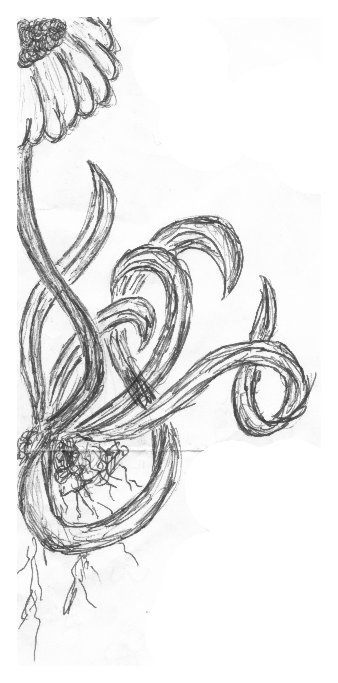
\includegraphics[width=3.5 cm]{Doodleflower}
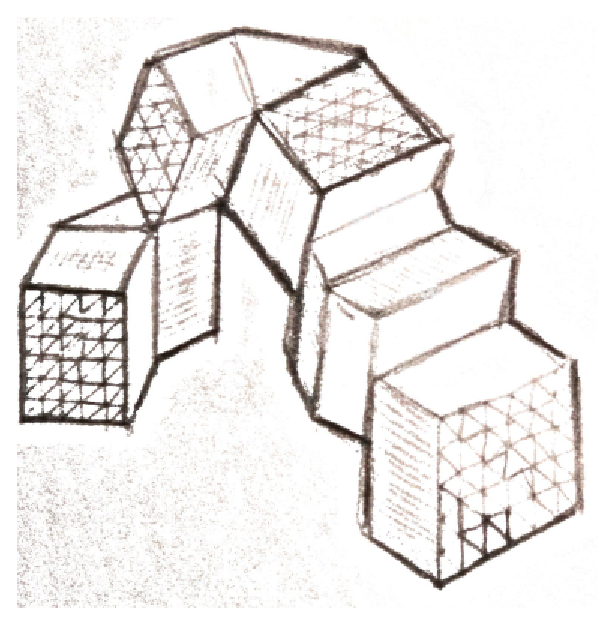
\includegraphics[width=5 cm]{Doodle1}
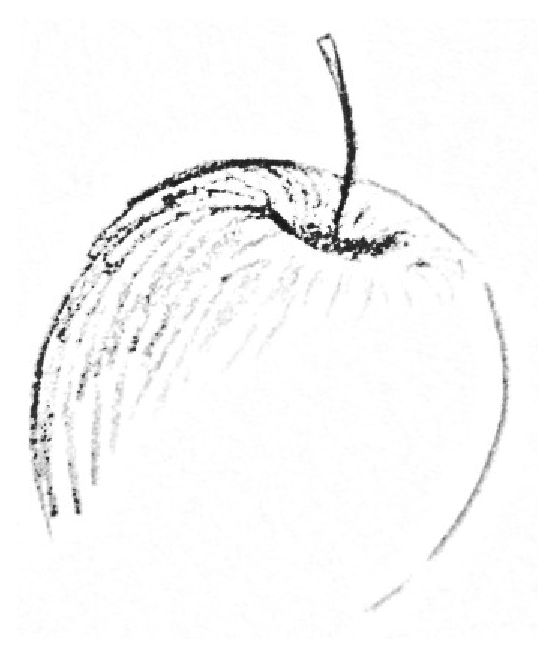
\includegraphics[width=5 cm]{Doodleapple}


{It is a well known fact that {drawing} and doodling activates our brain.\index{doodle}
  Find opportunities in everyday life to draw something, for instance while on a phone call.  
Ideally do this without supporting your arm}{(see Meta--cognitive Exercises)}.


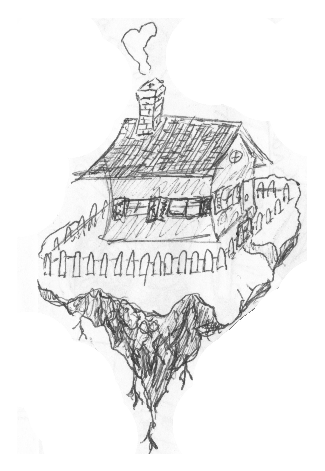
\includegraphics[width=5 cm]{Doodlehouse}
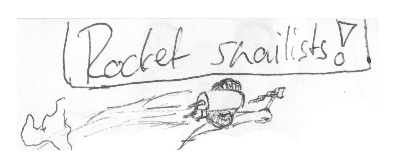
\includegraphics[width=8 cm]{Doodlesnail}

\end{document}